A storm surge refers to a significantly elevated water level along the coast, primarily occurring in combination with severe weather \citep{shoreline_management_guidelines}. Storm surges usually occur because of a combination or as a result of different factors such as wind-setup (the process of wind pushing water towards the coast), waves, lower atmospheric pressure (which can lead to local water rise), and in areas with tidal differences \citep{piecuch_high-tide_2022}.
In addition, the intensity and impact of a storm surge on a location depends on local conditions, including the orientation of the coast in relation to the wind direction and the morphology of the seabed and coast \citep{noaa_storm, shoreline_management_guidelines}.\\

In Denmark, the Wadden Sea and the west coast of Jutland are the most exposed areas, as the wind in Denmark primarily comes from the west \citep{cappelen_dmi_2020}, but the southeastern part of Denmark is also an exposed area. Over longer periods of westerly winds, the water in the North Sea will gradually be pushed into Kattegat and further down into the inner Danish waters. If a westerly wind is prolonged, the water will over time be pushed through the straits at Little Belt, Great Belt and Øresund and further into the Baltic Sea towards the Gulf of Bothnia \citep{kiesel_brief_2024, egusphere_baltic}. This phenomenon is called \textit{"preconditioning"} and describes how the water level rises in the Baltic Sea before the onset of a storm. Preconditioning is used as an indicator of a potential upcoming storm surge from the east \citep{kiesel_brief_2024, weisse_sea_2021}.\\

When the wind then decreases or changes to easterly, the accumulated water that has been pushed into the Baltic Sea will flow back towards the Danish Straits. This is called the \textit{"bathtub effect"} and is illustrated in figure \ref{Figur: Bathtub effect} \citep{kystdirektoratet_stormfloder, egusphere_baltic}. Due to the limited water volume in the southwestern part of the Baltic Sea and the narrow passages at straits of Denmark, a bottleneck effect occurs. This effect causes an accumulation of the water mass flowing from the Baltic Sea into the internal waters of Denmark. As a consequence, floods occur not only in Denmark, but also in adjacent fjords and bays in northern Germany and Southern Sweden \citep{egusphere_baltic, kiesel_brief_2024}.

\begin{figure}[H]
	\centering
	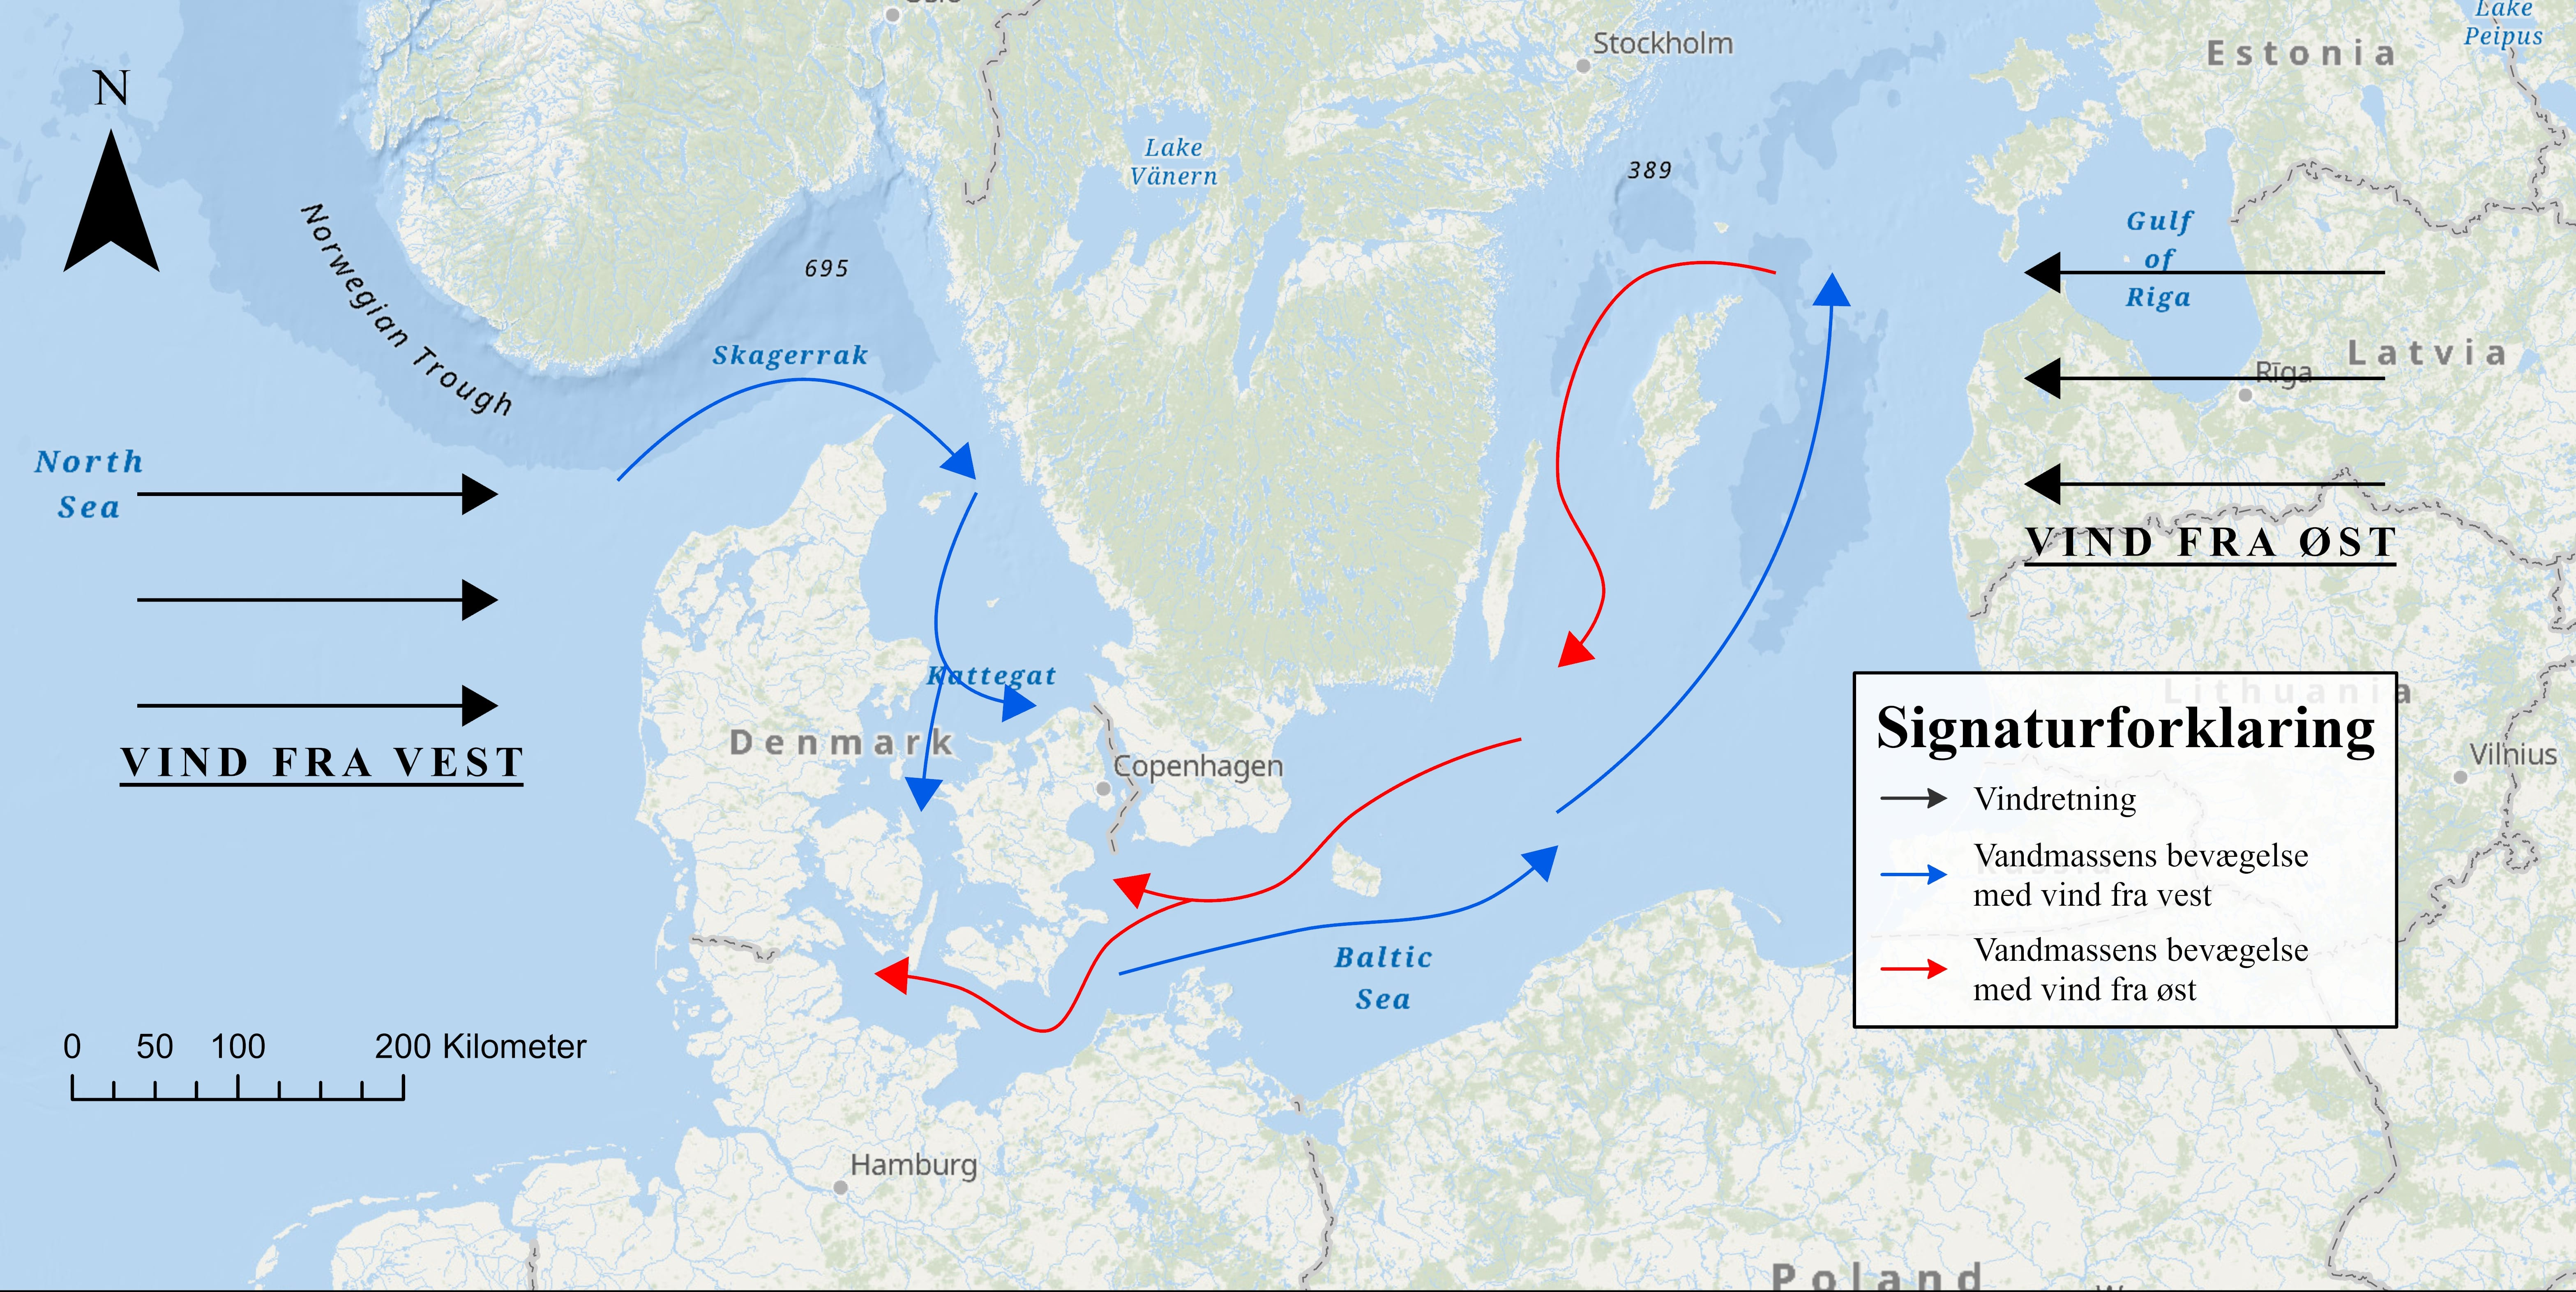
\includegraphics[width=0.8\linewidth]{images/teori/bathtub effect graphics.jpg}
	\caption{Illustration of the bathtub effect in the Baltic Sea. The black arrows indicate the wind direction and the blue and red arrows indicate the the movement of the water at westerly- and easterly winds respectively. Source: Own illustration, basemap from ESRI.}
	\label{Figur: Bathtub effect}
\end{figure}

Historically, several significant storm surges in Denmark, such as the storm surges of November 1872, November 2006 and October 2023, have been caused by a combination of prolonged westerly winds followed by easterly winds and the resulting bathtub effect \citep{kystdirektoratet_stormfloder}.

\subsection{October 2023 storm surge}
In the first half of October 2023, moderate wind conditions were observed with an average mean wind speed of 5.5 ms$^{-1}$ and an average maximum 10-minute mean wind speed of 18.3 ms$^{-1}$ from the west, which resulted in significant water transport through the Kattegat and further into the Baltic Sea \citep{dmi_vejrarkiv}. A few days before the storm surge, water levels were reported to be 20-50 cm higher than average in the bays of Kiel and Lübeck in Germany \citep{kiesel_brief_2024} and a storm surge event was expected to hit Southern Denmark and Northern Germany within the coming days.\\

On Wednesday, 18th of October, the wind direction changed to blow from the east (Figure \ref{Figur: Vinddata Danmark}) cause by pressure differences between a high pressure system over Northern Scandinavia and a low pressure system west of Great Britain, which formed a wind field and a pressure gradient over the Southern part of the Baltic Sea \citep{kiesel_brief_2024}. The mean wind speed in Denmark increased to 12.2 ms$^{-1}$ and the maximum 10-minute mean wind to 28.3 ms$^{-1}$ on the evening of October 20, 2023. In addition,the air pressure in Denmark dropped to around 995 hPa and a maximum gust of around 34 ms$^{-1}$ was measured. The event is therefore classified as hurricane strength \citep{dmi_vejrarkiv}.
\begin{figure} [H]
	\centering
	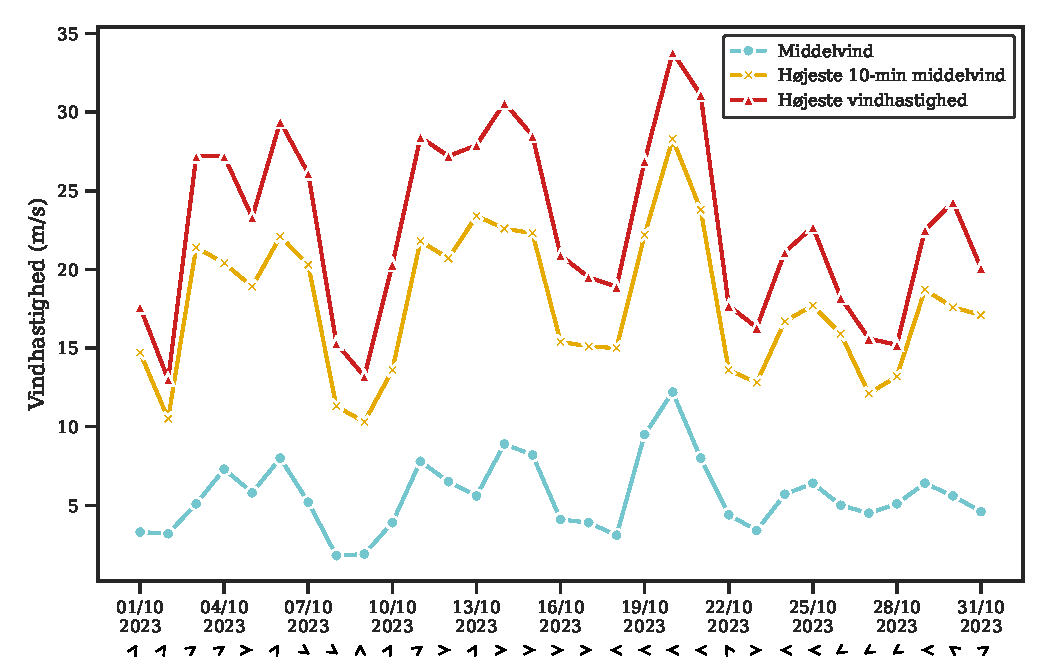
\includegraphics[width=0.9\linewidth]{images/teori/vinddata_grafer/Danmark_vinddata.pdf}
	\caption{Vinddata for Danmark i oktober 2023 der viser middelvind, højeste 10.min middelvind og højeste vindhastighed i m/s. De sorte pile i bunden indikerer hvilken retning vinden blæser imod. Kilde: Data fra \cite{dmi_vejrarkiv}.}
	\label{Figur: Vinddata Danmark}
\end{figure}

The combination of strong easterly winds and the large transportation of water into the Baltic Sea over a period of 15 days resulted, according to \cite{kystdirektoratet_stormflod2023}, significant increases in water levels in the internal waters of Southern Denmark during the afternoon and into the evening of October 20th. The highest official water level recorded was measured in Aabenraa Harbour at 2.16 metres above normal levels \citep{damberg_vaerste_2023}. The floods caused extensive damage to summer cottage areas, coastal areas, ports and cities \citep{kystdirektoratet_stormflod2023, naturskaderadet_anmeldelser_2023}.\\
The storm surge that hit Denmark also affected a number of the country's neighbours. Northern Germany and the southern part of Sweden also recorded elevated water levels and strong winds \citep{kiesel_brief_2024}. At the same time, Hurricane Babet was observed over Great Britain and the Republic of Ireland resulting in extreme rainfall over the British Isles \citep{met_office_storm_2023}.